% RECOMMENDED %%%%%%%%%%%%%%%%%%%%%%%%%%%%%%%%%%%%%%%%%%%%%%%%%%%
%%%%%%%%%%%%%%%%%%%%%%% file typeinst.tex %%%%%%%%%%%%%%%%%%%%%%%%%
%
% This is the LaTeX source for the instructions to authors using
% the LaTeX document class 'llncs.cls' for contributions to
% the Lecture Notes in Computer Sciences series.
% http://www.springer.com/lncs       Springer Heidelberg 2006/05/04
%
% It may be used as a template for your own input - copy it
% to a new file with a new name and use it as the basis
% for your article.
%
% NB: the document class 'llncs' has its own and detailed documentation, see
% ftp://ftp.springer.de/data/pubftp/pub/tex/latex/llncs/latex2e/llncsdoc.pdf
%
%%%%%%%%%%%%%%%%%%%%%%%%%%%%%%%%%%%%%%%%%%%%%%%%%%%%%%%%%%%%%%%%%%%


\documentclass[runningheads,a4paper]{llncs}

\usepackage{url}
\usepackage{tipa}

\usepackage{makeidx}         % allows index generation
\usepackage{graphicx}        % standard LaTeX graphics tool
                             % when including figure files
\usepackage[bottom]{footmisc}% places footnotes at page bottom

\usepackage{textcomp} % textdegree symbol

\hyphenation{Wiki-Talk}
\newcommand{\dbar}{\mbox{d\hspace{-.35em}\={}}}

% see the list of further useful packages
% in the Reference Guide

\makeindex             % used for the subject index
                       % please use the style svind.ist with
                       % your makeindex program

%%%%%%%%%%%%%%%%%%%%%%%%%%%%%%%%%%%%%%%%%%%%%%%%%%%%%%%%%%%%%%%%%%%%%%%%%%%%%%%%%%%%%%%%%

\begin{document}

\mainmatter  % start of an individual contribution

% first the title is needed
\title{DigiSami and Digital Natives: Interaction Technology for the North Sami Language}
% a short form should be given in case it is too long for the running head
\titlerunning{DigiSami and Digital Natives}
\toctitle{DigiSami and Digital Natives: Interaction Technology for the North Sami Language}

\author{Kristiina Jokinen\inst{1,2} \and Katri Hiovain\inst{1} \and Niklas Laxstr\"{o}m\inst{1}
        \and Ilona Rauhala\inst{1} \\ and Graham Wilcock\inst{1}}
\authorrunning{Jokinen, Hiovain, Laxstr\"{o}m, Rauhala and Wilcock}
%\authorrunning{Jokinen \textit{et al.}}
\tocauthor{Kristiina Jokinen, Katri Hiovain, Niklas Laxstr\"{o}m, Ilona Rauhala and Graham Wilcock}

\institute{University of Helsinki, Helsinki, Finland \\
\email{firstname.lastname@helsinki.fi}
\and University of Tartu, Estonia
}


\maketitle

\begin{abstract}
The DigiSami project operates in the general context of revitalisation of endangered languages, and focuses on the digital visibility and viability of the North Sami language in particular. The goal is to develop technological tools and resources that can be used for speech and language processing and for experimenting with interactive applications. Here we propose an interactive talking robot application as a means to reach these goals, and present preliminary analyses of a spoken North Sami conversational corpus as a starting point for supporting interaction studies. These are first steps in the development of SamiTalk, a Sami-speaking robot application which will allow North Sami speakers to interact with digital resources using their own language. The on-going work addresses the challenges of the digital revolution by showing that multilingual technology can be applied to small languages with promising results.
\end{abstract}

\keywords{language revitalisation \textperiodcentered\ digital resources \textperiodcentered\ interaction technology}

\section{Introduction}
\label{sec:introduction}

The digital revolution has made a dramatic impact on nearly all aspects of society. Global economics, technology and politics produce interdependence of countries world-wide, while everyday life is drastically changed by a media-rich
environment where communication technology brings people speaking different languages together in new ways.
New genres of discourse emerge through social media platforms and applications, collaboratively edited content, and user-generated online materials.
The role of language in the novel communicative situations is prominent, since language is the vehicle that manifests these changes.
On the other hand, the new technological paradigms affect language use as the language also adapts itself to these changes: by being frequently used in the new digital contexts,
the language adopts new functions and forms, and is thus able to maintain its suppleness and flexibility.
However, minority or lesser-used languages lack resources as well as speakers who could actively use the language in everyday and in novel communicative contexts, and they are thus most affected by these new paradigms in communication technology. The smaller language communities are the most sensitive to outside forces, and therefore also most endangered in the new digital world.

A language can survive only if it is in active use in a variety of interactive contexts, including social media networks, business and commerce, live literature/blogs, etc.
In other words, a language should be viable in the digital world: it needs to have a function that is performed digitally. In order to enable digital presence and have such a function, it is important to have tools and applications which support use of the language in the new communication paradigms, and in order to develop these, it is necessary to have high quality corpora and resources. However, cutting-edge enabler technologies of language processing applications are typically available only for widely-spoken languages (so called "comfort zone" languages), while smaller communities are often left to their own resources, or they need to translate or localise information that is unavailable in their native language. The needs of less-resourced languages are to be specifically considered, in order to reduce the unbalanced situation among languages, see \cite{Soria:ea:13}.

Nowadays much effort is directed to enable less-resourced languages to build necessary resources and to support their digital viability. Revitalisation of endangered languages is
done through various projects and workshops, community efforts, influencing legislation, teaching, and cultural activities. In this article we describe our work in the DigiSami project and discuss especially its goals to apply language and speech technologies, to support and revitalise the North Sami language community. We present a preliminary analysis of a spoken North Sami conversational corpus, and propose that an interactive talking robot application can make an important contribution towards the goals of the project.

The article is structured as follows.
Section~\ref{sec:digisami} presents the project goals to improve digital visibility and viability of the North Sami language. We also provide an overview of the Sami languages and of existing tools and resources for North Sami that can be used for speech and language processing.
Section~\ref{sec:digisami-corpus} describes the DigiSami Corpus of spoken North Sami and gives preliminary analyses of the conversations in terms of laughter, speech properties, and change in the function of adjective forms.
Section~\ref{sec:samitalk} describes first steps towards developing SamiTalk, a spoken dialogue system for Sami-speaking humanoid robots. Based on previous work on the WikiTalk system, SamiTalk will provide spoken information access from Sami Wikipedia. The DigiSami Corpus is being used to develop the speech components and to model dialogue.
Section~\ref{sec:conclusion} presents conclusions and future work.

\section{DigiSami and North Sami language resources}
\label{sec:digisami}

\subsection{The DigiSami project}
\label{sec:digisamiproject}

The DigiSami project, within its larger framework of Academy of Finland and Hungarian Science Academy cooperation, sets out to investigate how modern language technology and corpus-based linguistic research can contribute to facing digitalisation challenges with lesser-resourced Fenno-Ugric languages.
As described in \cite{Jokinen:LREC:14}, the DigiSami project focuses on North Sami, and aims to
\begin{itemize}
\item collect data from dialogue-related genres and annotate it on a range of levels from grammatical to discourse phenomena,
\item experiment with language technology applications that can strengthen the user's interest in using the language in various interactive contexts, focussing in particular on the SamiTalk application,
\item alleviate barriers in accessing information from user-generated content, supporting community-based generation of translated material on the web, based partially on existing language resources and technology.
\end{itemize}

This article concentrates on the first two goals of the project and describes how the SamiTalk robot application can be used to support revitalisation of the North Sami language. The robot application is chosen because it is an interface to collaboratively edited Wikipedia information (based on the WikiTalk application \cite{Wilcock:QACD:12,Jokinen:Wilcock:IWSDS:12}), and also, as a novel application, it is expected to increase the visibility of the languages by kindling interest in learning how the North Sami language can be used in the novel interactive technology (see discussion in Section~\ref{sec:samitalk}). In particular, it is expected that young people may become more interested in using and studying the language, which is an important and effective strategy for language revitalisation in general.

\subsection{The Sami languages}
\label{sec:sami-languages}

We have chosen North Sami as our target language, since it is the largest of the Sami languages and generally used as a lingua franca among the Sami people.
It is one of the Sami languages spoken in the area that extends from Middle Scandinavia to the Kola Peninsula, spanning four countries: Norway, Sweden, Finland, and Russia,
as shown on the map in Figure~\ref{fig:sami-map}.

\begin{figure}[htb]
\centering
\includegraphics[scale=.4]{saamimap_v0-1_JL.png}
%\includegraphics[scale=.4]{saamimap_v0-1_JL_data_collection.png}
\caption{The Sami language areas at the beginning of the 20th century. Source: \cite{Sammallahti:98}.
\newline So: South Sami, Um: Ume Sami, Pi: Pite Sami, Lu: Lule Sami, No: North Sami,
\newline In: Inari Sami, Sk: Skolt Sami, Ak: Akkala Sami (now extinct), Ki: Kildin Sami,
\newline Tr: Ter Sami.}
\label{fig:sami-map}
\end{figure}

%moved later: The Sami languages belong to the Fenno-Ugric branch of the Uralic language family, which also includes Finnish, Estonian, and Hungarian.

The Sami languages are divided into eastern and western groups, shown in Table~\ref{tab:languages}.
Both language groups are represented in Finland where North Sami, Inari Sami and Skolt Sami are spoken. All Sami languages are endangered, some even critically, although continuous efforts are made for their revitalisation and documentation.
%The last speaker of Akkala Sami died in 2003.

\begin{table} \center
\caption{The Sami languages, their estimated number of speakers in 2012 \cite{Gruenthal:Siegl:12} and their region (No: Norway, Sw: Sweden, Fi: Finland, Ru: Russia).}
\label{tab:languages}
\begin{tabular}{| l | l | } \hline
\textbf{Western Sami languages}           & \textbf{Eastern Sami languages} \\ \hline
South Sami (500 speakers) No, Sw          & Inari Sami (350 speakers) Fi \\ \hline
Ume Sami ($<$10 speakers) Sw              & Skolt Sami (300 speakers) Fi, Ru \\ \hline
Pite Sami (40 speakers) Sw                & Kildin Sami (700 speakers) Ru \\ \hline
Lule Sami (1000 speakers) No, Sw          & Ter Sami ($<$10 speakers) Ru \\ \hline
North Sami (30,000 speakers) No, Sw, Fi   &  \\ \hline
\end{tabular}
\end{table}

The Sami languages are close relatives and the distinction between a dialect and a language is sometimes vague. The differences mainly concern morphophonetic variation whereas syntactic changes are fairly small \cite{Palismaa:Eira:01}. The closer the languages are geographically, the more easily speakers understand each other, but also the majority language affects understandability since it is reflected in differences in both vocabulary and pronunciation (see more in Section~\ref{sec:majority-language}).

The Sami languages use the Latin alphabet with various diacritics to represent phonological differences. An exception is Kildin Sami which is spoken only in Russia and written using the Cyrillic alphabet. Although written Sami texts have existed for more than 200 years, their orthographies were irregular and were stabilised only in late 1970's when the Sami Council (then: the Nordic Sami Council) decided to adopt a new uniform orthography for North Sami spoken in Finland, Norway and Sweden  \cite{Kulonen:ea:05}. This coincides with national educational reforms in the 1970's and 1980's which gave a legal basis for the use of Sami language in education.

The normative work continues today in collaboration with representatives from all the relevant countries. However, even today older Sami speakers who did not learn to read and write in Sami at school may feel uncertain of the written language conventions. The different majority languages (Finnish, Norwegian, and Swedish) also have influence on the written language due to their different phonetic rules and orthographic conventions: it is not uncommon to find "mistakes" in crowd-sourced North Sami texts such as Wikipedia articles, due to irregularities in the way the words are spelled. This makes automatic processing of digital texts a challenge.

Nowadays the Sami language (the term used to refer collectively to all the Sami language variations and to emphasise the Sami as a nation) is officially recognised in Norway, Finland, and Sweden. The respective Language Acts (1992 in Finland and Norway, 2000 in Sweden) guarantee the official status of the Sami language and the right of the Sami to use the Sami languages in all official encounters. Moreover, as a result of the national education reform in Finland, the Basic Education Act 1998 entitles Sami children who live in the Sami Homeland area and speak the Sami language to receive the main part of their basic education in the Sami language.

\subsection{The North Sami language}
\label{sec:north-sami}

North Sami divides into three main dialects: Tornio, Finnmark and Sea Sami dialects, and the Finnmark dialect is further divided into western and eastern groups. The Finnmark dialect has the most speakers of North Sami, so the DigiSami corpus collection (see more in \ref{sec:digisami-corpus}) was conducted especially in the locations which are representative of the main Finnmark dialect variations (see the map in
Figure~\ref{fig:data-locations}).

Like all the Sami languages, North Sami belongs to the Fenno-Ugric branch of the Uralic language family, which also includes Finnish, Estonian, and Hungarian. Due to common origin and close contacts, North Sami shares many similarities especially with Finnish and Estonian, although the languages are rather distantly related. North Sami and Estonian resemble each other in morphophonological aspects, since both have a rich phoneme repertoire and complicated morpho-phonetic variations. While Finnish has preserved much of the original agglutinative marking in inflection, both Estonian and North Sami have changed over time towards fusional inflected morphology: instead of marking morphemes by suffixes only, the languages exploit phonetic modifications to the root, in particular consonant gradation which deals with consonant stem alternations between strong and weak grades.

The main linguistic similarities between Finnish and North Sami include the following \cite{Sammallahti:98}:

\begin{itemize}
\item Inflection with cases, persons, tense and mood,
\item Similar morpheme and word order,
\item Negation by using a negation verb as in Fenno-Ugric languages in general (except Estonian)
\item A number of common words, both from a common origin and through loans from Finnish to North Sami.
\end{itemize}

There are also many differences between North Sami and Finnish. For instance, compared with Finnish, North Sami has:

\begin{itemize}
\item Separate dual verb forms and pronouns in addition to singular and plural forms,
\item Six inflectional cases for nouns, as opposed to 15 in Finnish,
\item No vowel harmony, whereas Finnish features back/front vowel harmony (typical for Fenno-Ugric languages in general excluding Estonian)
\item Complex repertoire of phonemes and morphophonological variation:
\begin{itemize}
\item 31 consonants including voiced and voiceless nasals as well as pre-aspirated consonants and affricates. The latter are not found in the Finnish system of only 17 consonants.
\item Consonant gradation concerns all consonant phonemes, as opposed to Finnish where alternations always involve a stop at least in either grade (weak or strong). According to \cite{Sammallahti:98}, the number of stem gradation patterns in North Sami is counted to be at least 175.
\item The 5 vowels (/u, o, a, e, i/) do not contain front vowels /y/, /\"a/, and /\"o/ which are found in Finnish (however, these occur in recent loan words in North Sami, like \textit{fysihkka}), and some dialects do not distinguish between /a/ and /\"a/). The length of vowels is phonemic as in Finnish and Estonian.
\item Numerous diphthongs have phonetic length unlike Finnish and Estonian. North Sami also features triphthongs.
\end{itemize}
\end{itemize}


\subsection{Existing North Sami language resources}
\label{sec:resources}

Technical development has played a significant role in revitalising and modernising the Sami languages. Nowadays several language tools are available for speakers and language learners to check spelling, look for suitable words, and learn the language. Special keyboards adapted to the Sami orthographies are available for computers and cell-phones \cite{Tromso:keyboards}, so as to facilitate Sami language text input, which can be challenging due to various diacritics and their different encodings.

While the Sami languages have been fairly well documented and studied, North Sami enjoys a relatively favourable situation as it also has various tools for automatic language analysis. They have been developed at Giellatekno at University of Troms{\o} and are available from the website \cite{Tromso:analyzers}. For instance, the spell-checker \textit{Divvun} supports the writing of North Sami, and has an important role in taking the written language norms into use. Morphological and syntactic parsers for text corpora are also available, as well as a translation tool from North Sami to Norwegian Bokm\r{a}l and experimental translation systems to Finnish and to other Sami languages.

A new approach to Sami morphology is taken in \cite{Groenroos:ea:15} which studies how to use an Active Learning approach to morphological segmentation. Since high-quality morphological analyzers require a significant amount of expert labour, data-driven approaches may provide sufficient quality for many applications. \cite{Groenroos:ea:15} describes how the semi-supervised Morfessor FlatCat method is used to create a statistical model for morphological segmentation for a large unannotated corpus, with a small amount of annotated word forms which are selected using an active learning approach.

Revitalisation of a language also means gaining new speakers via language learning. For this there are digital dictionaries and also a language learning website \textit{Oahpa!} \cite{Tromso:oahpa}. It offers different ways to learn and test language skills, with exercises for testing and practising morphology, vocabulary and syntax. The digital dictionaries \cite{Tromso:dicts} include more updated vocabulary than printed ones, and it is possible to search for a word, both from a majority language to Sami and vice versa.

Various spoken and text corpora are also available in North Sami. These are at the Sami culture archive \cite{Oulu:archive} in the Giellagas Institute at University of Oulu. The collection of audio and video material as well as photographs and written documents supports research infrastructure and documentation of the Sami culture. The spoken corpora consist of interviews and official texts, such as the corpus of Yle
S\'apmi radio programs \cite{Oulu:aanitteet}, but there are no natural conversations in the corpora. However, the DigiSami project has collected a small corpus of spoken conversational data in North Sami (see
Section~\ref{sec:digisami-corpus}). The corpus has been transcribed and translated into Finnish, and is unique in that it contains spoken, non-scripted conversations between groups of people.

\subsection{Existing North Sami speech technology}

Current speech technology applications for the Sami languages still require development and are not yet commonly in use. However, advances have already been made in the development of a speech synthesizer and a speech recognizer for North Sami. A big challenge in the development is the limited speech corpora available. Some speech/voice data is available for North Sami under licence of the Sami Parliament of Norway, but speech corpora for other Sami languages remain in limited use at the moment.

A North Sami speech synthesizer \textit{North Sami Infovox 4} (Windows) or \textit{North Sami iVox} (OS X) was developed by Divvun and the Norwegian Sami Parliament, in cooperation with the voice and speech technology company Acapela \cite{Tromso:tale}.
%(\url{http://divvun.no/en/tale/tale.html}).
It was released in May 2015. The system has both a female and a male voice, and they can be adapted to the user's needs. North Sami speech synthesis has also been studied in the Simple4All project \cite{Simple4All}
%(\url{http://simple4all.org/})
which focuses on creating methods that enable speech synthesis systems to be built by little or no supervised learning from the data.

A North Sami speech recognizer has been developed in the DigiSami project in collaboration with our partners at Aalto University. \cite{Leinonen:15} describes building an automatic speech recognizer for North Sami and discusses its further development. This is a notable work since to the best of our knowledge, this is the first and only speech recognizer for any of the Sami languages today.

%leave out
%In addition to North Sami, there are some spoken language
%corpora in other Sami languages. Spoken corpus work is done
%at
%least for Skolt and Pite Sami. The Skolt Sami Documentation
%Project at Unversity of Helsinki \cite{Miestamo:ea:15} is
%analyzing and annotating Skolt Sami archive materials
%provided
%by the Institute for the Languages of Finland (Kotus). The
%Pite
%Sami Documentation Project at Humboldt-Universit\"{a}t zu
%Berlin
%collected an audio and video corpus of Pite Sami in 2008-2011
%\cite{Wilbur:14}.

\section{The DigiSami Corpus}
\label{sec:digisami-corpus}

The DigiSami Corpus of spoken North Sami consists of both read speech (257 minutes of annotated data) and conversations of two or three persons (195 minutes of annotated data). The speakers are all native speakers of North Sami, and their ages vary between 16 and 65 years. The corpus was collected in five locations that represent the main communities of the Finnmark variation of North Sami:
Enonteki\"{o}, Utsjoki, Inari and Ivalo in Finland, as well as Kautokeino and Karasjok in Norway. Figure~\ref{fig:data-locations} shows the locations for the data collection. More details about the collection and analysis of the corpus can be found in \cite{Jokinen:Wilcock:SLTU:14} and \cite{Jokinen:LREC:14}).

\begin{figure}[t]
\centering
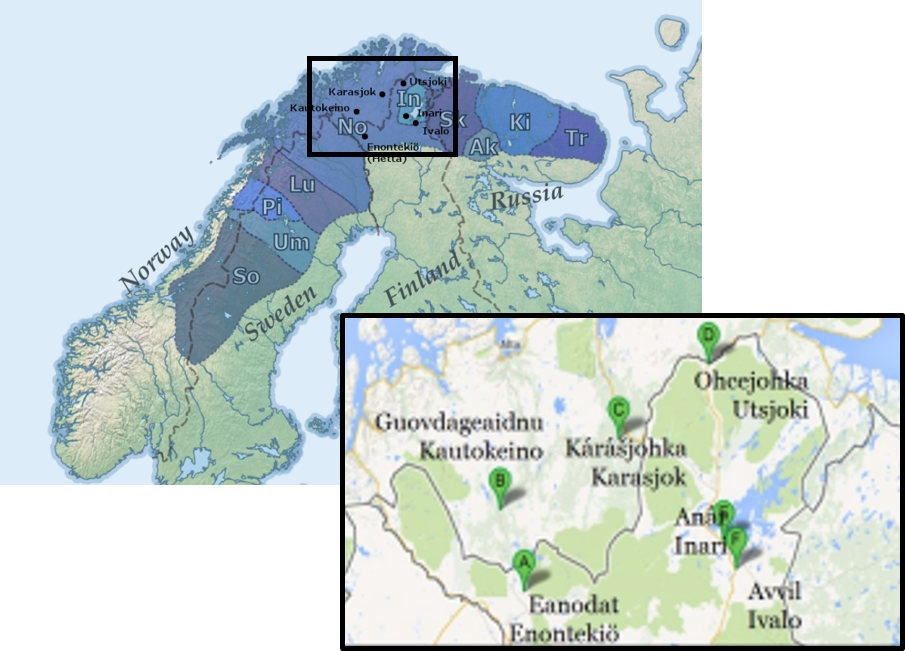
\includegraphics[width=1\linewidth]{DigiSamiCollectionLocations.png}
\caption{The DigiSami data collection locations.}
\label{fig:data-locations}
\end{figure}

The DigiSami corpus is unique among the Sami language corpora because it contains natural spoken conversations between groups of participants. The interlocutors discuss freely about their own interests but also about the Wikipedia articles they were to write (such as Sami language, Sami costume, music, reindeer herding, and snowmobiles). Conversations between young students concern their everyday life, and the topics include the next vacation, driving school, and cars. Two adult men, who have known each other for a long time, converse about translation between Sami and other languages, and venture on with the technological tools that have been made to help writing North Sami more correctly.

The styles of the conversations differ depending on the age of the speakers and their hierarchical status. Participants who are familiar with each other have casual conversations and they often refer to things they had been talking about earlier. The conversations between a pupil and a teacher, however, are more formal and resemble interviews rather than conversations; the topics stick to the forthcoming task, i.e. things that one could write a Wikipedia article about.

The DigiSami corpus is multimodal, i.e. conversations are both recorded and videotaped. Thus it is possible to study non-verbal as well as verbal communication. Furthermore, the spoken non-scripted conversations allow us to study the language as it is used, not as it should be in formal grammars and dictionaries, and thus it forms a basis for studies on spoken colloquial North Sami. Moreover, it helps to create a model of the North Sami language for the use of speech technology applications.

Below we briefly discuss three aspects of the on-going DigiSami corpus analysis: the participant's engagement and the role of laughter in interactions, the influence of the majority language on spoken North Sami, and the apparent change in the use of adjective forms in the present-day spoken North Sami.

\subsection{Preliminary analysis: engagement and interaction}

The annotation of the corpus was done with Praat and consists of 5 time-aligned tiers: a phonological/phonetic transcription, the words, the sentence in orthographic form, a Finnish translation, and remarks on things like dialectal variation. Challenges in the annotation included unclear speech, unknown proper names, as well as some insider jokes, besides some Norwegian words in the corpus collected in Norway.

The participants' engagement in the conversation and mutual bonding can be measured using multimodal and non-verbal cues, such as the amount of laughing or chuckling, and overlapping speech. The analysis of different types of laughter does not only show humour and joking, but also indicates connections to how well participants know each other, if they are nervous or embarrassed, and what kind of relationship they have with each other. Overlapping speech, on the other hand, indicates how involved the speakers are in contributing to the shared goal of the conversation. For the purposes of measuring this kind of engagement and studying the roles of laughing and overlapping speech in conversations, we annotated the data with these features on the remarks tier in Praat. The basic statistics are shown in Table~\ref{tab:laughter}.

\begin{table}\center
\caption{Laughter and overlapping speech}
\label{tab:laughter}
\begin{tabular}{| l | l | r | r |}
\hline
Conversation code & Informant code & Laughter & Overlapping speech    \\
  		     	  &                &          & \\
\hline
01\_S & S-1     &  9 & 15 \\
      & S-2     & 25 &  3 \\
      & S-3     &  9 &  4 \\ \hline
02\_V & V-1     & 75 &  1 \\
      & V-2     & 34 & -- \\
      & V-3     & 63 &  1 \\ \hline
03\_V & V-2     &  7 &  1 \\
      & V-3     &  6 & -- \\ \hline
04\_S & S-1     &  0 & -- \\
      & S-2     &  6 & -- \\
      & S-3     &  1 & -- \\ \hline
05\_TP & TP-2   & 21 & -- \\
       & TP-3   & 34 & -- \\ \hline
06\_PS & PS-1   &  5 & -- \\
       & PS-3   &  4 & -- \\ \hline
07\_SX & SX-1   &  3 & -- \\
       & SX-X   &  1 & -- \\ \hline
08\_VV & VV-Vih & 15 & -- \\
       & VV-Vio & 19 & -- \\ \hline
\end{tabular}
\end{table}

As can be seen, the number of laughter occurrences varies much depending on the dialogue, but interestingly, there is not much overlapping speech in the conversations, except
in \textit{01\_S}. For example, in the conversation \textit{02\_V}, in which the participants laugh and chuckle the most, there are only two occurrences of overlapping speech. This leads us to conclude that laughing and overlapping speech indeed have different functions in the conversations, and although they can both be regarded as signs of the interlocutors' engagement, the preconditions for their occurrence are different. In \textit{01\_S}, both laughter and overlapping speech signal similar positive engagement in the conversation, whereas in \textit{02\_V}, the participants seem nervous and their conversation topics change very fast. Despite the many laughs, there is practically no overlapping speech, which seems to indicate that the constant chuckling might be related to a relief of embarrassment and nervousness in the situation.
In fact, a closer analysis shows that although most of the instances in \textit{02\_V} are free or mirthful laughs, one fourth of them occurs when the speaker is embarrassed. This is in contrast with the conversation
\textit{01\_S}, where laughter is more evenly distributed among free and mirthful types, and embarrassed laughs are a small minority.

In our other study \cite{Hiovain:Jokinen:LREC:16}, we noticed that laughter is also related to the participants' social roles: lack of laughter may also indicate rather formal conversations and an asymmetrical relationship between the speakers, such as in teacher-pupil conversation. In other words, laughter creates mutual bonds among the interlocutors and reinforces shared experience even if the situation is embarrassing, whereas lack of laughter is often a signal of distancing relation.

In fluent conversations, where people know each other and show no impression of nervousness, both laughter and high amount of overlapping speech seem to indicate enthusiasm and close relationship, as well as elaborated coordination of the conversation by smooth turn-taking: laughter occurs when the participants share jokes or funny stories, and turn-taking is timed so as not to have long silences.

These observations will be substantiated with deeper analysis and statistical modelling. Precise conditions for turn-taking, laughing and generally positive attitude will be explored further so as to enable appropriate interaction models be implemented in the SamiTalk application. A useful case is for instance to be able to recognise the user's embarrassment or uncertainty, and alleviate such situations accordingly.

%Turn-taking was usually performed smoothly and the overall
%amount of overlapping speech was low. There was remarkable
%overlapping speech only in one fluent conversation with three %young female participants from Norway (see Table~\ref
%{tab:laughter}).
%This is a remarkable exception as in the other conversations %there was no overlapping speech.

\subsection{Preliminary analysis: influence of majority language}
\label{sec:majority-language}

North Sami is spoken in three countries: Finland, Norway and Sweden, and the language is thus in contact with a Baltic-Finnic language (Finnish) and with North Germanic (Scandinavian) languages (Norwegian and Swedish).
As discussed in \cite{Aikio:ea:14}, the fact that North Sami is spoken in three countries makes describing the variation of the language multidimensional. Different parts of the speech community are influenced by different majority languages, and practically all speakers are bilingual or even trilingual. Language contacts with majority languages have made a strong impact on dialect diversification, resulting in changes in various linguistic features. Such features include phonetics and intonation, syntax and lexical expansion with words which denote new concepts but do not follow the traditional dialectological analysis. Consequently, \cite{Aikio:ea:14} suggest a new way to classify the present-day dialects on the basis of both traditional regional features and the contact influence of the state language.

The DigiSami corpus indicates remarkable differences between Sami spoken in Norway and Finland, although dialectally the regions of Ivalo, Utsjoki and Karasjok, where the DigiSami conversation corpus was collected, represents the same eastern Finnmark dialect of North Sami. The differences can be heard in different pronunciation of various phonemes, most remarkably of \textipa{/r/}.
In our data from Karasjok in Norway, \textipa{/r/} has several allophones, occurring as \textipa{[\o]}, \textipa{[r]}, \textipa{[\*r]} and \textipa{[\textfishhookr]}, while in our data from Finland it occurs only as \textipa{[r]} with no allophonic variation. This allophonic variation seems to follow the patterns of the majority languages. The IPA transcriptions and spectrogram pictures from the speech of two young girls in Figures~\ref{fig:fertet-NO} and~\ref{fig:fertet-FI} demonstrate this difference (the example word is \textit{fertet} `have to').

The DigiSami conversations also exemplify differences in the influence of the majority languages on vocabulary. The use of Norwegian words in Sami spoken in Karasjok is much more common than the use of Finnish words in data collected in Ivalo and Utsjoki. In absolute counts the frequencies in the corpus are 60 vs 8 words, respectively.

\begin{figure}[htb]
%\sidecaption[t]
\includegraphics[scale=.65]{fertet-NO.png}
\caption{Sami spoken in Norway: \textipa{[f@{\*r}d\textlengthmark e\textlengthmark]}}
\label{fig:fertet-NO}
\end{figure}

\begin{figure}[htb]
%\sidecaption[t]
\includegraphics[scale=.65]{fertet-FI.png}
\caption{Sami spoken in Finland: \textipa{[fe\textlengthmark rht\textlengthmark e]}}
\label{fig:fertet-FI}
\end{figure}

An important reason to study the influence of the majority languages is that it affects the mutual comprehension more than the old regional dialect differences (see \cite{Sammallahti:98}). Especially different lexicon and idiomatic expressions have posed problems in cross-border communication between Finnish and Norwegian Sami speakers. Interestingly, these differences are often considered as interference rather than dialectal variation, although the features are already established in the language \cite{Aikio:ea:14}.

Using the acoustic language recognition technique of i-vector modelling, we studied if North Sami speech samples could be distinguished from each other automatically \cite{Jokinen:ea:Interspeech:16}. The average recognition error EER is 17.31\%, and the results support the view that the majority language has an impact on the dialect among bilingual speakers: mis-identification rates are significantly lower for Utsjoki and Ivalo than for Kautokeino and Karasjok. Moreover, since training of the recogniser was done with respect to a Finnish corpus, the better performance of the classifier for Ivalo and Utsjoki samples indicates their closed relation to Finnish. This research is important for the SamiTalk application, and
will be further used in enhancing speech recognition and other speech tools for North Sami.

\subsection{Preliminary analysis: adjectives in spoken language}

In North Sami the adjective attributive form tends to be different from the nominal predicate form, e.g.
\textit{fiinnis} (pred.) and \textit{fiinna} (attr.) `fine, nice', as in \textit{Beaivi lea fiinnis} `the day is nice') and \textit{Fiinna beaivi} `a nice day'.
The attributive marking system is complex \cite{Sammallahti:98}, and in practice, a speaker has to know both forms by heart. However, the DigiSami corpus shows that use of adjectives in spoken language often differs from what is presented in grammars and dictionaries, and the speakers use attribute forms in nominal predicate position and vice versa. The preliminary findings seems to indicate that the adjective system is changing, and that the main factor affecting the preservation of the form is the frequency of an adjective in a certain position.

For example, the adjective \textit{o{\dbar}as} `new' has the attributive form \textit{o{\dbar}{\dbar}a}, and its base form \textit{o{\dbar}as} is also used as the nominal predicate form. The adjective has 8 occurrences in the corpus, of which 6 occur in attributive position. The adjective occurs only twice as nominal predicate, and in both cases, the speaker sounds seemingly hesitant of the correct form. In one of these cases, the speaker hesitates and is looking for the right form, while in the other case, the speaker actually produces the attributive form \textit{o{\dbar}{\dbar}a}, which is wrong as the nominal predicate form. Another example is the adjective \textit{v\'attis} `difficult' which has the opposite distribution: the adjective occurs 5 times as a nominal predicate and once as an attribute, which occurrence has a wrong form.

The change in adjective attribute system has been recognized in other Sami languages \cite{Riessler:06}, such as South Sami \cite{Bergsland:94}. Our examples of non-normative use of adjectives forms may indicate a change in the adjective attribute system also in North Sami. The fact that the preserved form seems to depend on the frequency of the adjective form allows us to hypothesize that the change may be triggered by the frequency of the adjective in a certain position: it is plausible that adjectives such as `new'
\textit{o{\dbar}{\dbar}a} are more frequently used as attributes and thus tend to lose their nominal predicate form, whereas adjectives such `difficult' \textit{v\'attis} are used mostly as nominal predicates and thus tend to lose their attribute form. On the other hand, the cause for the change may also be due to an influence of the majority language: neither Finnish nor Norwegian distinguishes adjective forms based on their syntactic function.
Interestingly, it seems that the age of a speaker does not affect the use of the forms.

However, more data is essential in order to produce a reliable view of the adjective system and its change. Also further analysis of the changing mechanism is crucial for deeper understanding of language evolution in general. However, observations of the changing adjective system are crucial for producing good language models in order to develop speech applications such as SamiTalk.

\section{Towards SamiTalk: a Sami-speaking robot application}
\label{sec:samitalk}

Robot applications are leaving the research laboratories and reaching the general population,
both in homes and outside home. For example, WikiTalk \cite{Wilcock:QACD:12,Jokinen:Wilcock:IWSDS:12} is a multilingual spoken dialogue system that runs on a Nao robot.
The user and the robot have a dialogue in which the robot talks fluently about an unlimited range of topics using information from Wikipedia.

The DigiSami project is working towards the creation of SamiTalk, an interactive robot application in the North Sami language, as part of its support for language revitalisation using speech and language technologies.
The SamiTalk application will be based on existing WikiTalk technology
%\cite{Jokinen:Wilcock:IWSDS:12}
and will provide access to Sami Wikipedia information via a dialogue in North Sami with a humanoid robot.
This work is described in more detail by \cite{Wilcock:ea:IWSDS:16}.

Localisation \cite{Laxstrom:ea:IWSDS:16} of robot applications to an endangered language benefits the language in multiple ways. As mentioned in Section~\ref{sec:digisamiproject} this can provide motivation to use the language in novel communication framework. Localised robot applications can have a favourable effect on the prestige of the language, by showing that efforts have been made to support the language in the new technology.
For instance, at home, applications such as WikiTalk can prevent bottom-to-top language death by encouraging use of the language in the family.

Of course, with a multilingual application there is a risk that the users will just switch it to some other language, or even more likely, will not switch it to the local language from the default language, because they do not know how, or do not even know that their language is available. For this reason, language selection as a crucial function in localisation \cite{Laxstrom:ea:IWSDS:16} for robot applications is an important topic to study further.

New technology also offers opportunities for language revitalisation including existing or proposed Wikipedias for endangered languages. Wikipedias can bring together speakers of endangered languages even if they are not physically close to each other, can give motivation by Wikipedia's mission to provide free knowledge to everyone \cite{Wikipedia:motivation}
%(\url{http://wikipapers.referata.com/wiki/Motivation})
and can foster collaboration between speakers and scholars studying the endangered language. There is a risk, however, that a Wikipedia started by scholars may fail to attract native speakers, for example if they are unable to access Wikipedia via desktop computers or mobile devices.

Up to now, the available Wikipedias in the languages supported by WikiTalk have been very large. English Wikipedia has almost 5 million articles, Japanese Wikipedia has almost 1 million articles and Finnish Wikipedia has over 350,000 articles. In these languages, WikiTalk can talk about almost any topic the user is interested in. By contrast Sami Wikipedia is much smaller, with about 7000 articles.
This means that there are many topics that SamiTalk will not be able to talk about using existing methods. To address this problem, the DigiSami project is supporting initiatives to encourage the North Sami community to create new articles in Sami Wikipedia \cite{Jokinen:Wilcock:SLTU:14}, and is investigating methods for on-line translation of Wikipedia articles \cite{Laxstrom:ea:EAMT:15} into under-resourced languages.

%\subsection{Dialogue models}
%overview of dialogue models and presentation of the SamiTalk interaction.
% See KJ email if this is needed

\section{Conclusions and future work}
\label{sec:conclusion}

Often endangered languages face a gradual language death by assimilation. The ability to use one's own language with new technology, in the modern world, is almost a necessity to prevent gradual language death. In these cases the motivation to continue using the endangered language is a most important factor.

In this article, we have discussed revitalisation of North Sami, and presented our work within the DigiSami project, the goal of which is to support North Sami digital natives and their communication in the North Sami language in new digital contexts.
We are taking steps to address these issues by developing SamiTalk, an interactive robot application for an endangered language, North Sami. This application is based on the existing WikiTalk system. We have also collected a conversational spoken language corpus for North Sami. The DigiSami corpus has been transcribed and annotated, and preliminary analysis already shows interesting properties concerning laughing and joking, as well as turn-taking and overlapping speech. The corpus also provides examples of non-normative use of adjectives, which leads to a preliminary hypothesis that the alleged change in the North Sami adjective system is taking place, and that the frequency of an adjective in certain syntactic function affects the preservation of the form.

To develop a robust SamiTalk system, further work is required especially on the speech interface: comprehensive speech components for North Sami are needed for enabling natural conversations, and more spoken data is needed to cover language variation. We are developing speech technology for the language with our collaborators. Future work will deal with integration of the speech components on the robot, as well as deeper analysis of the conversational corpus.


\subsection*{Acknowledgement}
The work is funded by the Academy of Finland through the project Fenno-Ugric Digital Citizens
(grant n\textdegree270082). The first author would also like to thank support of the Estonian Science Foundation project
(grant n\textdegree IUT 20-56).

%\newpage

%\nocite{Paggio:ea:10}
\bibliographystyle{splncs03_unsort}
%\bibliography{../digisami}

\begin{thebibliography}{10}
\providecommand{\url}[1]{\texttt{#1}}
\providecommand{\urlprefix}{URL }

\bibitem{Soria:ea:13}
Soria, C., Mariani, J., Zoli, C.: Dwarfs sitting on the giants' shoulders --
  how {LTs} for regional and minority languages can benefit from piggybacking
  major languages. In: Norris, M., Anonby, E., Junker, M.O., Ostler, N.,
  Patrick, D. (eds.) Proceedings of XVII FEL Conference. pp. 73--79. Ottawa
  (2013)

\bibitem{Jokinen:LREC:14}
Jokinen, K.: Open-domain interaction and online content in the {Sami} language.
  In: Calzolari, N., Choukri, K., Declerck, T., Loftsson, H., Maegaard, B.,
  Mariani, J., Moreno, A., Odijk, J., Piperidis, S. (eds.) Proceedings of Ninth
  International Conference on Language Resources and Evaluation (LREC 2014).
  European Language Resources Association (ELRA), Reykjavik (2014)

\bibitem{Wilcock:QACD:12}
Wilcock, G.: {WikiTalk}: A spoken {Wikipedia}-based open-domain knowledge
  access system. In: Proceedings of the COLING 2012 Workshop on Question
  Answering for Complex Domains. pp. 57--69. Mumbai (2012)

\bibitem{Jokinen:Wilcock:IWSDS:12}
Jokinen, K., Wilcock, G.: Multimodal open-domain conversations with the {Nao}
  robot. In: Mariani, J., Rosset, S., Garnier-Rizet, M., Devillers, L. (eds.)
  Natural Interaction with Robots, Knowbots and Smartphones: Putting Spoken
  Dialogue Systems into Practice, pp. 213--224. Springer (2014)

\bibitem{Sammallahti:98}
Sammallahti, P.: The Saami Languages: An Introduction. {Davvi Girji},
  K\'{a}r\'{a}\v{s}johka (1998)

\bibitem{Gruenthal:Siegl:12}
Gr\"unthal, R., Siegl, F.: Uralilaisten kielten pensasmalli ja arvioidut
  puhujam{\"a}{\"a}r{\"a}t ({The "bush model" of the Uralic languages and the
  estimated numbers of speakers}), {Department of Finno-Ugric Studies,
  University of Helsinki} (2012)

\bibitem{Palismaa:Eira:01}
Palismaa, M., Eira, I.M.G.: {Gielas gillii, mielas millii 9 -
  Davvis\'{a}megiela suopmanat (From language to language, from mind to mind 9
  - The dialects of North Sami)}. {Davvi Girji}, K\'{a}r\'{a}\v{s}johka (2001)

\bibitem{Kulonen:ea:05}
Kulonen, U.M., Seuruj{\"a}rvi-Kari, I., Pulkkinen, R. (eds.): The Saami - A
  Cultural Encyclopedia. Suomalaisen Kirjallisuuden Seura, Helsinki (2005)

\bibitem{Tromso:keyboards}
{Divvun, University of Troms{\o}}: Keyboards (2015),
  \url{http://divvun.no/keyboards/index.html}, [Online; accessed
  2-December-2015]

\bibitem{Tromso:analyzers}
{Giellatekno, University of Troms{\o}}: Programs for analysing {North Saami}
  (2015), \url{http://giellatekno.uit.no/cgi/d-sme.eng.html}, [Online; accessed
  2-December-2015]

\bibitem{Groenroos:ea:15}
{Gr\"onroos}, S.A., Jokinen, K., Hiovain, K., Kurimo, M., Virpioja, S.:
  Low-resource active learning of {North S{\'a}mi} morphological segmentation.
  {Presentation at First International Workshop on Computational Linguistics
  for the Uralic Languages, Troms{\o}, Norway} (2015)

\bibitem{Tromso:oahpa}
{Divvun, University of Troms{\o}}: Welcome to the {OAHPA!} portal (2015),
  \url{http://oahpa.no}, [Online; accessed 2-December-2015]

\bibitem{Tromso:dicts}
{Giellatekno, University of Troms{\o}}: {North Saami} dictionaries (2015),
  \url{http://dicts.uit.no/smedicts.eng.html}, [Online; accessed
  2-December-2015]

\bibitem{Oulu:archive}
{Giellagas Institute, University of Oulu}: {The Saami Culture Archive of
  University of Oulu} (2015),
  \url{http://www.oulu.fi/giellagasinstitute/the_saami_culture_archive},
  [Online; accessed 2-December-2015]

\bibitem{Oulu:aanitteet}
{Giellagas Institute, University of Oulu}: {A. {\"A}{\"a}nitteet (Recordings)}
  (2015), \url{http://www.oulu.fi/giellagasinstituutti/aanitteet}, [Online;
  accessed 2-December-2015]

\bibitem{Tromso:tale}
{Divvun, University of Troms{\o}}: Text-to-speech (2015),
  \url{http://divvun.no/en/tale/tale.html}, [Online; accessed 2-December-2015]

\bibitem{Simple4All}
{Simple4All Consortium}: {Simple4All}: developing automatic speech synthesis
  technology (2015), \url{http://simple4all.org/}, [Online; accessed
  2-December-2015]

\bibitem{Leinonen:15}
Leinonen, J.: Automatic Speech Recognition for Human-Robot Interaction Using an
  Under-Resourced Language. Master's thesis, Aalto University, School of
  Electrical Engineering, Department of Signal Processing and Acoustics, Espoo
  (2015)

\bibitem{Jokinen:Wilcock:SLTU:14}
Jokinen, K., Wilcock, G.: Community-based resource building and data
  collection. In: Proceedings of 4th Workshop on Spoken Language Technologies
  for Under-resourced Languages (SLTU-2014). pp. 201--206. St. Petersburg
  (2014)

\bibitem{Hiovain:Jokinen:LREC:16}
Hiovain, K., Jokinen, K.: Acoustic features of different types of laughter in
  {North Sami} conversational speech. In: Gilmartin, E., Campbell, N. (eds.)
  Proceedings of the LREC 2016 Workshop "Just Talking - Casual Talk among
  Humans and Machines". pp. 16--20. Portoroz (2016)

\bibitem{Aikio:ea:14}
Aikio, A., Arola, L., Kunnas, N.: Variation in {North Saami}. In: Smakman, D.,
  Heinrich, P. (eds.) Globalising Sociolinguistics: Challenging and Expanding
  Theory, pp. 243--255. Routledge (2014)

\bibitem{Jokinen:ea:Interspeech:16}
Jokinen, K., Trung, N.T., {Hautam\"aki}, V.: Variation in spoken {North Sami}
  language. In: Proceedings of INTERSPEECH 2016. San Francisco (2016)

\bibitem{Riessler:06}
Rie{\ss}ler, M.: Om samiskans attributive adjektivform. In: Amft, A., Svonni,
  M. (eds.) {S\'{a}pmi} Y1K. Livet i samernas {bos\"{a}ttningsomr\r{a}de}
  {f\"{o}r} ett tusen {\r{a}r} sedan, pp. 135--150. {S\'{a}mi} dutkan 3.
  {Ume\r{a}}: {Ume\r{a}} universitet (2006)

\bibitem{Bergsland:94}
Bergsland, K.: Sydsamisk grammatikk. Second edition. {Davvi Girji}, Karasjok
  (1994)

\bibitem{Wilcock:ea:IWSDS:16}
Wilcock, G., {Laxstr\"om}, N., Leinonen, J., Smit, P., Kurimo, M., Jokinen, K.:
  {Towards SamiTalk: a Sami-speaking Robot linked to Sami Wikipedia}. In:
  Proceedings of Seventh International Workshop on Spoken Dialogue Systems
  (IWSDS 2016). Saariselk{\"a} (2016)

\bibitem{Laxstrom:ea:IWSDS:16}
{Laxstr\"om}, N., Wilcock, G., Jokinen, K.: Internationalisation and
  localisation of spoken dialogue systems. In: Proceedings of Seventh
  International Workshop on Spoken Dialogue Systems (IWSDS 2016).
  Saariselk{\"a} (2016)

\bibitem{Wikipedia:motivation}
Wikipedia: Motivation (2015),
  \url{http://wikipapers.referata.com/wiki/Motivation}, [Online; accessed
  2-December-2015]

\bibitem{Laxstrom:ea:EAMT:15}
{Laxstr\"om}, N., Giner, P., Thottingal, S.: Content translation: Computer
  assisted translation tool for {Wikipedia} articles. In: Proceedings of 18th
  Annual Conference of the European Association for Machine Translation. pp.
  194--197 (2015)

\end{thebibliography}

\end{document}
